\documentclass{article}
\usepackage{graphicx}
\usepackage{subcaption}
\usepackage{caption}
\usepackage[margin=0.5in]{geometry}
\usepackage{float}

\title{Encoding 01110010}
\author{Welby Seely}
\date{9/9/2025}

\begin{document}
    \pagenumbering{gobble} % disable page numbering

% --- Title page only ---
    \begin{titlepage}
        \centering
        \vspace*{\fill}   % push content to vertical center
        {\LARGE \bfseries Encoding 01110010 \par}
        \vspace{1em}
        {\LARGE \bfseries Welby Seely \par}
        \vspace{1em}
        {\LARGE \bfseries 9/9/2025 \par}
        \vspace*{\fill}
    \end{titlepage}

% --- Figures start on page 2 ---
    \begin{figure}[H]
        \centering

        % Row 1 (2 items)
        \begin{subfigure}{0.49\textwidth}
            \centering
            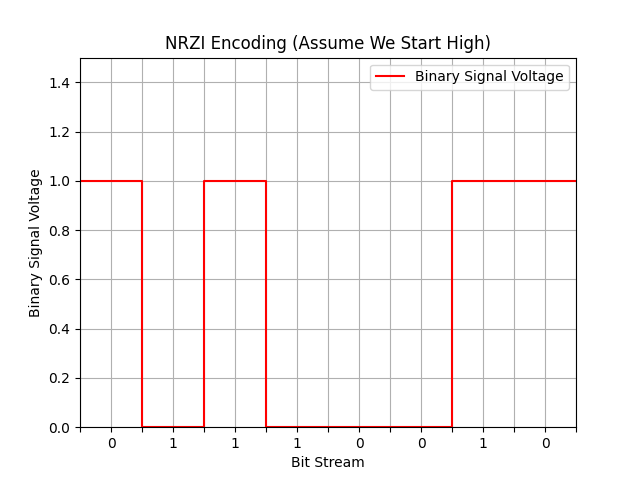
\includegraphics[width=\linewidth]{nrz}
            \caption{NRZ (Active Low)}
        \end{subfigure}
        \hfill
        \begin{subfigure}{0.49\textwidth}
            \centering
            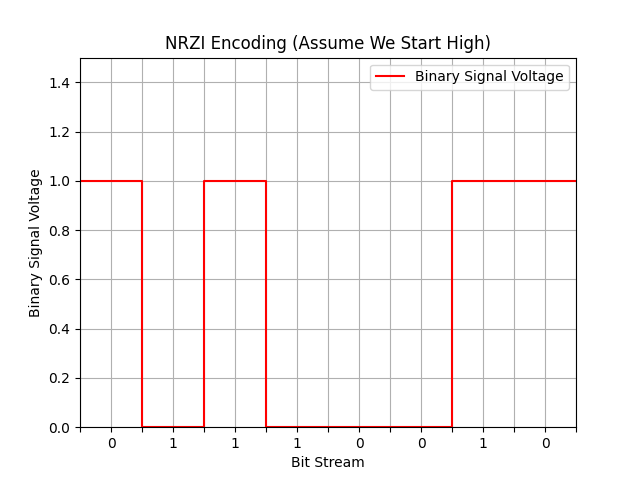
\includegraphics[width=\linewidth]{nrzi}
            \caption{NRZI}
        \end{subfigure}

        \bigskip

        % Row 2 (2 items)
        \begin{subfigure}{0.49\textwidth}
            \centering
            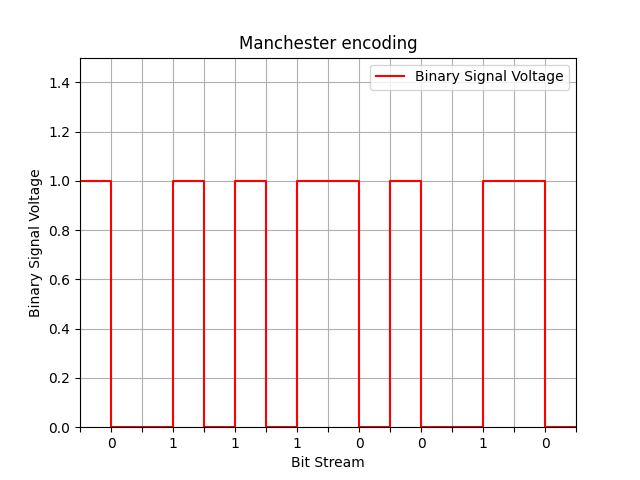
\includegraphics[width=\linewidth]{manchester}
            \caption{Manchester}
        \end{subfigure}
        \hfill
        \begin{subfigure}{0.49\textwidth}
            \centering
            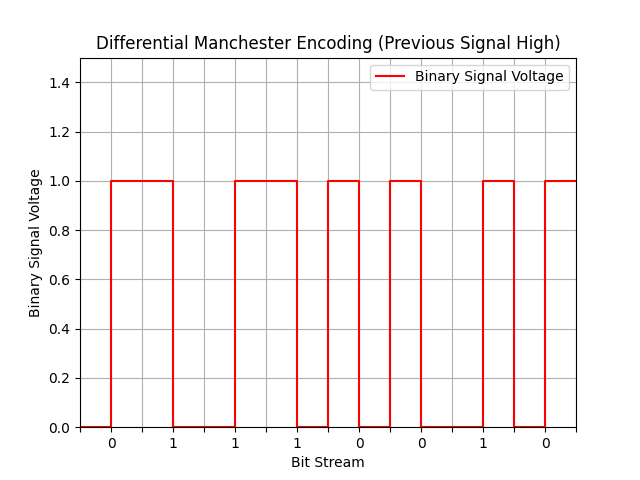
\includegraphics[width=\linewidth]{differential_manchester}
            \caption{Differential Manchester}
        \end{subfigure}

        \bigskip

        % Row 3 (1 item, centered and wide)
        \begin{subfigure}{0.7\textwidth}
            \centering
            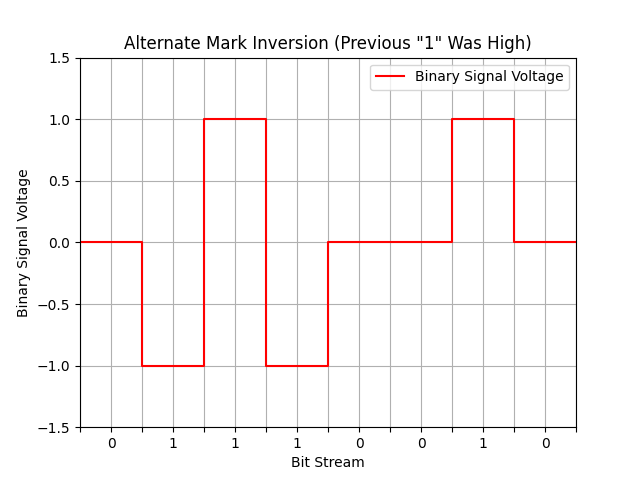
\includegraphics[width=\linewidth]{ami}
            \caption{AMI}
        \end{subfigure}

        \caption{NRZ, NRZI, Manchester, Differential Manchester, and AMI.}
    \end{figure}

\end{document}
